\chapter{Espaces de Sobolev}\label{Ch-Sobo}\index[aut]{Sobolev (Sergueï Lvovitch), 1908-1989, Russe}
\begin{abstract}
Les espaces de Sobolev sont des espaces fonctionnels.
Plus précisément, un espace de Sobolev est un espace vectoriel de fonctions muni de la norme
obtenue par la combinaison de la norme~$L^p$ de la fonction elle-même ainsi que de ses
dérivées jusqu'à un certain ordre.
Les dérivées sont comprises dans un sens faible, au sens des distributions afin de rendre l'espace complet.

Les espaces de Sobolev sont donc des espaces de Banach.
Intuitivement, un espace de Sobolev est un espace de Banach ou un espace de Hilbert de fonctions pouvant
être dérivées suffisamment de fois (pour donner sens par exemple à une équation aux dérivées
partielles) et muni d'une norme qui mesure à la fois la taille et la régularité de la fonction.

Les espaces de Sobolev sont un outil très important et très adapté à l'étude des équations aux
dérivées partielles. En effet, les solutions d'équations aux dérivées partielles, appartiennent plus
naturellement à un espace de Sobolev qu'à un espace de fonctions continues dont les dérivées
sont comprises dans un sens classique (mais rien n'empêche d'avoir de la chance).
\end{abstract}

\medskip
\begin{histoire}%
Le \textsc{xx}\fup{e} siècle avait commencé par la thèse de Lebesgue\index[aut]{Lebesgue (Henri-Léon), 1875-1941, Français}
 <<~intégrale, longueur, aire~>> qui constitue vraiment le début de la théorie de la mesure.
%Par la suite, de nouvelles intégrales sont créées sur les traces de Lebesgue (intégrales
%de Denjoy, de Perron et d'Henstock...). La théorie de la mesure finit par rejoindre la
%théorie des probabilités qui est axiomatisée en 1933 par Kolmogorov.
La théorie de Lebesgue mène à l'étude des espaces~$L^p$, qui permettront,
sur les traces de Hilbert,\index[aut]{Hilbert (David), 1862-1943, Allemand}
Riesz\index[aut]{Riesz (Frigyes), 1880-1956, Hongrois}
 et Banach,\index[aut]{Banach (Stephan), 1892-1945, Polonais}
 l'étude des opérateurs différentiels.

\sbox{\MaBoiteAvecPhotos}{\setlength{\tabcolsep}{0pt}\scriptsize%
\begin{tabular}{cccc}
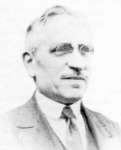
\includegraphics[height=\the\HauteurDesPhotos]{Lebesgue3}&
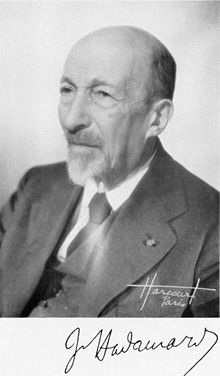
\includegraphics[height=\the\HauteurDesPhotos]{Hadamard}&
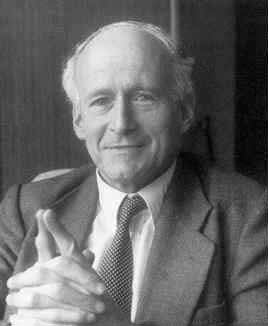
\includegraphics[height=\the\HauteurDesPhotos]{Schwartz}&
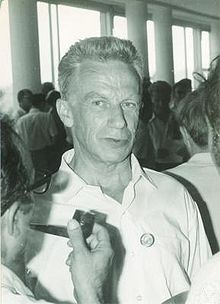
\includegraphics[height=\the\HauteurDesPhotos]{Sobolev}\\
Lebesgue &Hadamard &Schwartz &Sobolev%
\end{tabular}}
\medskip
\ImageADroite{%\ifVersionDuDocEstVincent\begin{cutout}{0}{0.50\linewidth}{0pt}{8}\else\begin{cutout}{0}{0.44\linewidth}{0pt}{8}\fi
Cauchy\index[aut]{Cauchy (Augustin Louis, baron -), 1789-1857, Français}
 avait publié nombre d'applications de sa théorie dans des recueils d'exercices, notamment
concernant l'évaluation d'intégrales réelles, qu'il n'hésita pas à généraliser en ce qu'on appelle
aujourd'hui la <<~valeur principale de Cauchy~>>, un peu moins d'un siècle avant que Hadamard\index[aut]{Hadamard (Jacques Salomon), 1865-1963, Français}
 en ait besoin dans sa résolution des équations aux dérivées partielles dans un problème d'hydrodynamique par les <<~parties finies~>> et
que Laurent Schwartz\index[aut]{Schwartz (Laurent), 1915-2002, Français}
 n'en vienne aux distributions.}

\medskip
L'étude des conditions de régularité des solutions des équations aux dérivées partielles permet à Sergueï Sobolev\index[aut]{Sobolev (Sergueï Lvovitch), 1908-1989, Russe} et ses continuateurs de définir ses espaces de fonctions et les théorèmes de trace en fonction des
propriétés géométriques du domaine.
\end{histoire}
\colorblack

\medskip
\section{Distributions}\index{distribution}
Une distribution (également appelée fonction généralisée) est un objet qui généralise
la notion de fonction et de mesure.
La théorie des distributions étend la notion de dérivée à toutes les fonctions localement
intégrables et au-delà.

\medskip
\begin{definition}[Espace des fonctions tests~$\mathcal{D}(\Omega)$]
Soit~$\Omega$ un sous-espace topologique de~$\RR^n$ (ou~$\CC^n$).
\textcolorblue{L'espace des fonctions tests~$\mathcal{D}(\Omega)$} est l'ensemble des fonctions
à valeurs réelles indéfiniment dérivables de~$\Omega$ à support compact inclus dans~$\Omega$.

On munit cet espace vectoriel de la topologie suivante: un ensemble~$U \subset \mathcal{D}(\Omega)$ est
ouvert ssi~$\forall K \subset \Omega$ compact et~$f \in U$ dont le support est inclus dans~$K$,
il existe~$\epsilon > 0$ et~$k \ge 0$ tels que:
\begin{equation}
  \{ g \in \mathcal{D}(\Omega)\;\mid\; \operatorname{supp}(g) \subset K\quad\text{ et }\quad\forall x \in K,\; |f^{(k)}(x)-g^{(k)}(x)|\le \epsilon \}\;\subset\;U.
\end{equation}
Muni de cette topologie, $\mathcal{D}(\Omega)$ est un espace vectoriel topologique \textcolorred{non métrisable}.
\end{definition}

\medskip
\begin{definition}[Distribution]
\textcolorblue{Une distribution} est une \textbf{forme linéaire continue}\index{Forme!linéaire}
sur~$\mathcal{D}(\Omega)$.
\end{definition}

L'ensemble des distributions est donc le dual topologique de~$\mathcal{D}(\Omega)$ et est donc noté~$\mathcal{D}'(\Omega)$.\index{espace!dual topologique d'un espace vectoriel}
%%%%%%%%%%%%%%%%%%
\medskipvm
Toujours aussi classiquement, si~$T$ est une distribution et~$\varphi$ une fonction test de
$\mathcal{D}(\Omega)$ alors on note~$T(\varphi)=\langle T,\varphi \rangle$. (i.e.
$\langle\cdot,\cdot\rangle$ désigne comme d'habitude le crochet de dualité).
%%%%%%%%%%%%%%%%%%
\medskipvm
Dans~$\mathcal{D}'(\mathbb{R})$, l'application qui à~$\varphi$ associe~$\varphi(0)$ est une distribution et c'est la distribution de Dirac\index{distribution!de Dirac}\index[aut]{Dirac (Paul Adrien Maurice), 1902-1984, Anglais}:
\begin{equation}
\langle\delta,\varphi\rangle=\varphi(0)
\end{equation}
%%%%%%%%%%%%%%%%%%
\medskipvm
Une propriété fondamentales est que \textcolorblue{toute fonction localement intégrable~$f$ représente aussi
une distribution~$T_f$ définie par la forme intégrale suivante}:
\begin{equation}
  \langle T_f,\phi\rangle=\int_{\mathbb{R}}f(x)\phi(x)\,\dd x, \quad \forall \phi\in\mathcal{D}(\Omega)
\end{equation}


\medskip
\section{Dérivées au sens des distributions}\index{dérivée!au sens des distributions}
Pour définir la dérivée d'une distribution, considérons d'abord le cas d'une fonction différentiable
et intégrable~$f:\mathbb{R}\rightarrow\mathbb{R}$.
Soit~$\varphi$ une fonction test, supposée régulière et à support compact.
Une intégration par parties permet d'écrire:
\begin{equation}
  \int_\RR f'(x) \varphi(x)\,\dd x = -\int_\RR f(x)\varphi'(x)\,\dd x \qquad\text{ soit }\qquad I_{f'}(\varphi)=I_{-f}(\varphi')
\end{equation}
En effet, puisque la fonction~$\varphi$ est nulle en dehors d'un ensemble borné (elle est à support
compact), les termes de bords s'annulent.

\medskip
\begin{definition}[Dérivée d'une distribution]
Si~$S$ est une distribution, cet exemple suggère que l'on puisse \textcolorblue{définir sa dérivée~$S'$ comme
la forme linéaire} qui à une fonction test~$\varphi$ fait correspondre la valeur~$- S(\varphi')$.
On pose donc:
\begin{equation}\colorred
  \langle S', \varphi \rangle = - \langle S, \varphi' \rangle
\end{equation}
Cette définition étend la notion classique de dérivée:
chaque distribution devient \textcolorred{indéfiniment dérivable} et l'on peut montrer les
propriétés usuelles des dérivées.
\end{definition}

\medskip
Cette notion peut aussi se définir comme la dérivée du produit de dualité~$\langle S,\varphi\rangle$.
On note~$\varphi_h:x\rightarrow\varphi(x-h)$ la translatée de~$\varphi$ par la valeur~$h\in{\mathbb R}$,
alors, en utilisant la linéarité et la continuité par rapport au deuxième terme:
\begin{equation}
\langle\frac{\dd S}{\dd x},\varphi\rangle= \lim_{h\rightarrow 0}\frac{ \langle S,\varphi_h\rangle- \langle S,\varphi\rangle}{h}
= \langle S,\lim_{h\rightarrow 0} \frac{\varphi_h-\varphi}{h} \rangle= -\langle S,\frac{\dd\varphi}{\dd x}\rangle
\end{equation}
Lorsque la distribution~$S$ modélise un phénomène physique, la fonction test~$\varphi$ peut
s'interpréter comme un instrument de mesure, $\langle S,\varphi\rangle$ en étant le résultat;
la définition ci-dessus représente alors la mesure expérimentale (au moins de pensée) de la
dérivée du phénomène~$S$ à l'aide de l'instrument~$\varphi$.

\medskip
\textcolorgris{Nous définirons dans un autre cours (sur le traitement du signal) les notions de
distribution à support compact, les distributions tempérées et la décroissance rapide utiles en
analyse de Fourier ainsi que les espaces de Schwartz.}





\medskip
\section{Espaces~$W^{m,p}(\Omega)$}\index{espace!de Sobolev~$W^{m,p}(\Omega)$}\index[aut]{Sobolev (Sergueï Lvovitch), 1908-1989, Russe}

\begin{definition}[Espace~$W^{m,p}(\Omega)$]
Soient~$\Omega \subset \RR^n$ un ouvert quelconque, $p$ un réel tel que~$1\leqslant p\leqslant \infty$
et~$m$ un entier naturel positif.
On définit l'espace de Sobolev~$W^{m,p}(\Omega)$ par:
\begin{equation}\label{Eq-SoboW}\colorred
W^{m, p}(\Omega)=\{u\in L^p(\Omega); D^\alpha u \in L^p(\Omega)\}
\end{equation}
où~$\alpha$ est un multi-indice tel que~$0\leqslant |\alpha| \leqslant m$ , $D^\alpha u$ est une
dérivée partielle de~$u$ au sens faible (i.e. au sens des distributions) et~$L^p$ un espace de Lebesgue.
\end{definition}

\medskip
La norme sur~$W^{m,p}(\Omega)$ est:\index{norme!sur~$W^{m,p}(\Omega)$}
\begin{equation}
\| u \|_{W^{m, p}} = \begin{cases} \left( \sum \limits_{0\leqslant | \alpha | \leqslant m} \| D^{\alpha} u \|_{L^{p}}^{p} \right)^{1/p}, & 1 \leqslant p < + \infty; \\ \max\limits _{0\leqslant | \alpha | \leqslant m} \| D^{\alpha} u \|_{L^{\infty}}, & p = + \infty; \end{cases}
\end{equation}
où~$\|\cdot\|_{L^{p}}$ désigne la norme des espaces de Lebesgue.
Muni de cette norme~$W^{m,p}(\Omega)$ est un espace de Banach.\index{espace!de Banach}
Dans le cas où~$p<\infty$, c'est aussi un espace séparable.
%%%%%%%%%%%%%%%%%%%%
\medskipvm
La norme:
\begin{equation}
\| u \|_{W^{m, p}} = \begin{cases} \sum\limits _{0\leqslant | \alpha | \leqslant m} \| D^{\alpha} u \|_{L^{p}}, & 1 \leqslant p < + \infty; \\ \sum\limits _{0 \leqslant | \alpha | \leqslant m} \| D^{\alpha} u \|_{L^{\infty}}, & p = + \infty. \end{cases} \end{equation}
est une norme équivalente à la précédente.
On utilisera donc indifféremment l'une de ces normes, et on notera la norme
employée~$\|\cdot\|_{W^{m, p}}$ ou plutôt~$\|\cdot\|_{m, p}$.

\medskip\colorgris
Si~$p<\infty$, alors~$W^{m,p}(\Omega)$ est identique à la fermeture de l'ensemble
$\lbrace u \in C^m(\Omega) ; \left\|u \right\|_{m,p} < \infty \rbrace$ par rapport à la norme
$\left\|\cdot\right\|_{m,p}$ où~$C^m(\Omega)$ désigne l'espace de H\"older des fonctions de
classe~$m$ sur~$\Omega$.
%%%%%%%%%%%%%%%%
\medskipvm
Le théorème de Meyers-Serrin~$H=W$ donne une définition équivalente, par complétion de l'espace
vectoriel normé:
\begin{equation}
\{u\in C^\infty(\Omega);\| u \|_{H^{m, p}} < \infty\}\quad\text{ avec }\quad
\| u \|_{H^{m, p}}:= \left( \sum_{| \alpha | \leqslant m} \| D^{\alpha} u \|_{L^{p}}^p \right)^{1/p}
\end{equation}
où~$D^\alpha u$ est une dérivée partielle de~$u$ au sens classique ($u \in C^\infty(\Omega)$).
\colorblack


\medskip
\section{Espaces~$H^m(\Omega)$}\index{espace!de Sobolev~$H^m(\Omega)$}\index[aut]{Sobolev (Sergueï Lvovitch), 1908-1989, Russe}

\begin{definition}[Espace~$H^m(\Omega)$]
\textcolorblue{Dans le cas~$p=2$, on note~$H^m(\Omega)$ l'espace~$W^{m,2}(\Omega)$, défini par la relation (\ref{Eq-SoboW}).}
\end{definition}

\medskip
Les espaces de Sobolev~$H^m$ ont un intérêt particulier car il s'agit alors d'\textcolorred{espaces de Hilbert.}\index{espace!de Hilbert}\index[aut]{Hilbert (David), 1862-1943, Allemand}
Leur norme est induite par le produit intérieur suivant:\index{Produit scalaire!de~$H^m(\Omega)$}
\begin{equation}(u,v)_{m} =\sum \limits _{0 \leqslant \vert \alpha\vert\leqslant m} \left( D^{\alpha} u, D^{\alpha} v\right)
\end{equation}
où: 
\begin{equation}(u,v) = \int_{\Omega} u(x) \overline{v}(x)\, \dd x
\end{equation}
est le produit intérieur dans $L^{2} ( \Omega)$; produit scalaire dans le cas réel, hermitien\index[aut]{Hermite (Charles), 1822-1901, Français} dans le cas complexe.

\medskip
\textcolorgreen{Si~$\Omega$ est Lipschitzien, alors l'ensemble~$C^\infty(\overline{\Omega})$ des
fonctions régulières jusqu'au bord de~$\Omega$ est dense dans~$H^m(\Omega)$.}

\medskip\colorgris
De plus, dans le cas où la transformation de Fourier peut être définie dans~$L^{2} ( \Omega)$ ,
l'espace~$H^k(\Omega)$ peut être défini de façon naturelle à partir de la transformée de Fourier
(voir cours sur le traitement du signal).
%%%%%%%%%%%%%%%%%%%%
\medskipvm
Par exemple si~$\Omega = \RR^{n}$, si~$\widehat{u}$ est la transformée de Fourier de~$u$:
\begin{equation}
H^{m}\left( \RR ^{n}\right)=\lbrace u \in L^{2}\left( \RR^{n}\right);\; \int_{\RR^{n}}\vert\hat{u}\left( \xi\right) \xi^{\alpha}\vert ^{2}\dd\xi \;<\infty
\end{equation}
pour $\vert\alpha\vert \leqslant m \rbrace$, ou ce qui est équivalent:
\begin{equation}
H^{m}\left( \RR ^{n}\right)=\left\lbrace u \in L^{2}\left( \RR^{n}\right);\; \int_{\RR^{n}}\vert\hat{u}\left( \xi\right) \vert ^{2}\left( 1+\xi^{2}\right)^{m} \dd\xi \;<\infty \right\rbrace
\end{equation}
et que:
\begin{equation}
(u,v)_{m}=\int_{\RR^{n}}\hat{u}(\xi) \overline{\hat{v}(\xi)} \left(1 + \xi^{2} \right) ^{m} \dd\xi
\end{equation}
est un produit hermitien\index[aut]{Hermite (Charles), 1822-1901, Français} équivalent à celui défini plus haut. Encore, si~$\Omega =\intoo{0}{1}$, on vérifie que:
\begin{equation}
H^m(\intoo{0}{1}) = \left\{ u\in L^2(\intoo{0}{1});\sum\limits_{n=-\infty}^{+\infty} (1+n^2 + n^4 + \dotsb + n^{2m}) |\widehat{u}_n|^2 < \infty \right\}
\end{equation}
où~$\widehat{u}_n$ est la série de Fourier de~$u$.
On peut aussi utiliser la norme équivalente:
\begin{equation}
\|u\|^2=\sum\limits_{n=-\infty}^{+\infty} (1 + |n|^{2})^m |\widehat{u}_n|^2
\end{equation}
\colorblack




\medskip
\section{Espaces~$H^m_0(\Omega)$}\index{espace!de Sobolev~$H_0^m(\Omega$}\index[aut]{Sobolev (Sergueï Lvovitch), 1908-1989, Russe}

\begin{definition}[Espace~$H^m_0(\Omega)$]
On définit \textcolorblue{$H^m_0(\Omega)$} comme l'adhérence dans~$H^m(\Omega)$
de~$\mathcal{D}(\Omega)$, ensemble des fonctions de classe~$C^\infty$ et à support compact
dans~$\Omega$.
\end{definition}
Plus exactement et de manière générale, $W^{m,p}_0$ est l'adhérence de~$\mathcal{D}(\Omega)$ dans l'espace
$W^{m,p}$. La définition ci-dessus correspond donc au cas~$p=2$.

\medskip
\begin{remarque}
Il faut bien comprendre que cela signifie quelque chose de simple: c'est l'ensemble constitué des
fonctions qui sont à la fois~$\mathcal{D}(\Omega)$ et~$H^m(\Omega)$.
Comme on s'intéresse à la frontière (puisque l'on prend l'adhérence), et que~$\Omega$ est un
ouvert, la valeur que prennent les fonctions de cet ensemble sur la frontière est celle
que prennent les fonctions de classe~$C^\infty$ et à support compact dans~$\Omega$,
soit~$0$ !
\end{remarque}

\textcolorgreen{Ainsi, <<~physiquement~>> les espaces~$H^m_0(\Omega)$ sont les fonctions
de~$H^m(\Omega)$ qui sont nulles sur~$\Gamma=\partial\Omega$, ainsi que leurs dérivées <<~normales~>>
jusqu'à l'ordre~$m-1$.}\index{dérivée!normale}
Plus mathématiquement, on dit que ces fonctions sont de trace nulle sur la frontière, comme par exemple:
\begin{equation}
  H_0^2(\Omega)=\left\{v / v\in H^2(\Omega), v|_\Gamma=0,
  \frac{\partial v}{\partial n}|_\Gamma=0\right\}
\end{equation}
Les espaces trace sont définis plus loin.\index{espace!trace}.
%%%%%%%%%%%%%%%%%%
\medskipvm
\textcolorred{Les espaces~$H^m_0(\Omega)$ sont des espaces de Hilbert.}\index{espace!de Hilbert}\index[aut]{Hilbert (David), 1862-1943, Allemand}


\medskip
\section{Espaces~$H^{-m}(\Omega)$}\index{espace!de Sobolev~$H^{-m}(\Omega)$}\index[aut]{Sobolev (Sergueï Lvovitch), 1908-1989, Russe}

\colorgris
Il est possible de caractériser le dual topologique de~$H^m_0(\Omega)$ de la façon suivante.\index{espace!vectoriel (topologique)}

$\forall m\ge 1$, on définit l'espace des distributions suivant:
\begin{equation}
H^{-m}(\Omega) =\left\{
f\in \mathcal{D}'(\Omega), f=\dsum_{|\alpha|\le m} \partial^\alpha f_\alpha,
\text{ avec } f_\alpha\in L^2(\Omega)
\right\}
\end{equation}
muni de la norme:\index{norme!sur~$H^{-m}(\Omega)$}
\begin{equation}
\|f\|_{H^{-m}} = \inf \left( \dsum_{|\alpha|\le m} \|f_\alpha\|^2_{L^2} \right)^{1\over2}
\end{equation}
l'infimum étant pris sur toutes les décompositions possibles de~$f$ sous la forme intervenant
dans la définition de~$H^{-m}$.
%%%%%%%%%%%%%%%%%
\medskipvm
Ainsi défini, l'espace~$H^{-m}(\Omega)$ est un espace de Hilbert isomorphe au dual
topologique de~$H^m_0(\Omega)$, et le crochet de dualité s'écrit:\index{espace!dual topologique d'un espace vectoriel}
\begin{equation}
\langle f,u\rangle_{H^{-m},H_0^m} = \dsum_{|\alpha\le m} (-1)^\alpha \dint_\Omega
f_\alpha \partial^\alpha u \dd x,
\quad \forall f\in H^{-m}(\Omega),\quad \forall u\in H^m_0(\Omega)
\end{equation}
Cette formule ne dépend pas de la décomposition de~$f$ en somme des~$\partial^\alpha f_\alpha$.
%%%%%%%%%%%%%%%%%%%%%
\medskipvm
Remarquons que le dual de~$H^m(\Omega)$ n'est pas un espace de distribution et ne possède
donc pas de caractérisation aussi simple.
\colorblack

\medskip
\section{Trace}\index{espace!trace}
Dans ce paragraphe, nous essayons de présenter la notion de trace de manière simple et intuitive.

\medskip
\textcolorgreen{Afin de pouvoir parler de la valeur d'une fonction sur la frontière de~$\Omega$,
il nous faut définir le prolongement (la trace) d'une fonction sur ce bord.}

\medskip
Cas~$n=1$:
on considère un intervalle ouvert~$I =]a;b[$ borné. On a vu que~$H^1(I)\subset C^0(\overline{I})$.
Donc, pour~$u\in H^1(I)$, $u$ est continue sur~$[a;b]$, et~$u(a)$ et~$u(b)$ sont bien définies.

\medskip
Cas~$n>1$:
il nous faut définir la trace lorsque l'on n'a plus~$H^1(I)\subset C^0(\overline{I})$.
On procède ainsi:
\begin{itemize}
  \item On définit l'espace:
	\begin{equation}C^1(\overline{\Omega}) = \left\{\varphi:\Omega\rightarrow\RR/ \exists O
	\text{ ouvert contenant } \overline{\Omega}, \exists \psi\in C^1(O), \psi_{|\Omega}=\varphi
	\right\}\end{equation}
	$C^1(\overline{\Omega})$ est donc l'espace des fonctions~$C^1$ sur~$\Omega$, prolongeables
	par continuité sur~$\partial\Omega$ et dont le gradient est lui-aussi prolongeable par continuité.
	Il n'y a donc pas de problème pour définir la trace de telles fonctions.
  \item On montre que, si~$\Omega$ est un ouvert borné de frontière~$\partial\Omega$
	<<~assez régulière~>>, alors~$C^1(\overline{\Omega})$ est dense dans~$H^1(\Omega)$.
  \item L'application linéaire continue, qui à toute fonction~$u$ de~$C^1(\overline{\Omega})$
	associe sa trace sur~$\partial\Omega$, se prolonge alors en une application linéaire continue
	de~$H^1(\Omega)$ dans~$L^2(\partial\Omega)$, notée~$\gamma_0$, qu'on appelle
	\textcolorblue{application trace}. On dit que~$\gamma_0(u)$ est la trace de~$u$ sur
	$\partial\Omega$.
\end{itemize}
Pour une fonction~$u$ de~$H^1(\Omega)$ qui soit en même temps continue sur~$\overline{\Omega}$,
on a évidemment~$\gamma_0(u) = u_{|\partial\Omega}$. \textcolorred{C'est pourquoi on note souvent par abus
simplement~$u_{|\partial\Omega}$ plutôt que~$\gamma_0(u)$.}

\medskip
De manière analogue, on peut définir~$\gamma_1$, l'application trace qui permet de
prolonger la définition usuelle de la dérivée normale sur~$\partial\Omega$.
Pour~$u\in H^2(\Omega)$, on a~$\partial_iu\in H^1(\Omega)$, $\forall i=1,\ldots,n$ et
on peut donc définir~$\gamma_0(\partial_iu)$. La frontière~$\partial\Omega$
étant <<~assez régulière~>> (par exemple, idéalement, de classe~$C^1$),
on peut définir la normale~$n = (n_1,\ldots,n_n)^T$ en tout point de~$\partial\Omega$.
On pose alors:
\begin{equation}\gamma_1(u) = \dsum_{i=1}^n \gamma_0(\partial_iu)n_i\end{equation}
Cette application continue~$\gamma_1$ de~$H^2(\Omega)$ dans~$L^2(\partial\Omega)$)
permet donc bien de prolonger la définition usuelle de la dérivée normale.
Dans le cas où~$u$ est une fonction de~$H^2(\Omega)$ qui soit en même temps
dans~$C^1(\overline{\Omega})$, la dérivée normale au sens usuel de~$u$ existe,
et~$\gamma_1(u)$ lui est évidemment égal.
\textcolorred{C'est pourquoi on note souvent, par abus, $\partial_n u$ plutôt que~$\gamma_1(u)$.}

\medskip
\section{Espace trace}\index{espace!trace}\index[aut]{Sobolev (Sergueï Lvovitch), 1908-1989, Russe}

\textcolorgreen{Compte tenu du paragraphe précédent qui exposait la notion
de trace, cette section n'a plus vraiment d'intérêt si l'on ne souhaite pas entrer trop
dans les détails mathématiques.}

\medskip
Dans le cas d'exposant entier, on note souvent l'ordre avec la lettre~$m$,
dans le cas non-entier, on utilisera la lettre~$s$, et donc les espaces seront notés:~$W^{s,p}$ ou~$H^s$.

\medskip
\subsection{Cas~$p=2$ et~$\Omega=\RR^{n}$}

\colorgris
Dans ce cas, l'espace de Sobolev~$H^{s}(\RR^n)$, $s\geqslant 0$, peut être défini grâce
à la transformée de Fourier:
\begin{equation}
H^{s} (\RR^n) = \left\{ u \in L^{2}(\RR^n) \colon \int_{\RR^n} ( 1 + | \xi |^{2} )^{s} | \hat{u} (\xi) |^{2} \, \dd\xi < + \infty \right\}.
\end{equation}
$H^{s}(\RR^n)$ est un espace de Hilbert muni de la norme:
\begin{equation}\| u \|_{H^{s}}^{2} = \int_{\RR^n} ( 1 + | \xi |^{2} )^{s} | \hat{u} (\xi) |^{2} \, \dd\xi \end{equation}
\colorblack

\medskip
\subsection{Cas~$p=2$ et~$\Omega \subset \RR^{n}$ quelconque}
On peut alors caractériser les espaces de Sobolev d'ordre fractionnaire~$H^s(\Omega)$
grâce au produit intérieur donné par:
\begin{equation}
(u, v)_{H^{s} (\Omega)} = (u,v)_{H^{k} (\Omega)} + \sum_{| \alpha | = k} \int_{\Omega} \int_{\Omega} \frac{( D^{\alpha}u (x) - D^{\alpha}u (y) ) (D^{\alpha}v (x) - D^{\alpha}v (y) )}{| x - y |^{n + 2 t}} \, \dd x \dd y
\end{equation}
où~$s = k + T$, $k$ est un entier tel que~$0 < T < 1$ et~$n$ est la dimension du domaine
$\Omega \subset \RR^{n}$.
La norme induite est essentiellement l'analogue pour~$L^2$ de la continuité au sens de H\"older.

\medskip
\subsection{Cas~$p\neq 2$ et~$\Omega = \intoo{0}{1}$}

\colorgris
On définit un opérateur~$D^s$ de dérivation d'ordre fractionnaire~$s$ par:
\begin{equation}
D^{s}u=\sum_{n=-\infty}^\infty (in)^s\widehat{u}(n)\mathrm{e}^{int}
\end{equation}

En d'autres mots, il s'agit de prendre la transformée de Fourier, de la multiplier par~$(in)^s$ et
à prendre la transformée de Fourier inverse (les opérateurs définis par la séquence:
transformation de Fourier --- multiplication --- transformation inverse de Fourier sont appelés des
multiplicateurs de Fourier).
Cet opérateur permet de définir la norme de Sobolev de~$H^s(\intoo{0}{1})$ par:
$\|u\|_{s,p}=\|u\|_p+\|D^s u\|_p$ et de définir l'espace de Sobolev~$H^s(\intoo{0}{1})$
comme l'espace des fonctions pour lesquelles cette norme est finie.
\colorblack

\medskip
\subsection{Cas général des espaces~$H^s$}\index[aut]{Sobolev (Sergueï Lvovitch), 1908-1989, Russe}

Soit~$s > \frac{1}{2}$. Si~$\Omega$ est un ouvert dont la frontière~$\partial \Omega$ est
<<~suffisamment régulière~>>, alors on peut définir un \textcolorblue{opérateur de trace~$T$}
qui à une fonction~$u \in H^{s}(\Omega)$ lui associe sa trace, i.e sa restriction sur la
frontière de~$\Omega$: \textcolorgreen{$Tu=u|_{\partial \Omega}$.}

Une hypothèse simple qui satisfasse la condition de régularité est que~$\partial \Omega$
soit uniformément~$C^m$ pour~$m \geqslant s$.
Ainsi défini, cet opérateur de trace~$T$ a pour domaine de définition~$H^s(\Omega)$ et
son image est précisément~$H^{s-1/2}(\partial \Omega)$.

En fait, $T$ est d'abord défini pour les fonctions indéfiniment dérivables et cette définition
est ensuite étendue par continuité à tout l'ensemble~$H^s(\Omega)$.
De façon intuitive, on peut dire que l'on perd en régularité <<~une demi-dérivée~>> en prenant
la trace d'une fonction de~$H^s(\Omega)$.

\textcolorgreen{Nous nous servirons de ces espaces dans le cas des éléments finis pour un problème
de continuité des contraintes à une interface entre deux milieux solides ayant des propriété
matérielles différentes. Ce problème sera abordé plusieurs fois dans ce document, et le
paragraphe~\ref{Sec-interf} fera une synthèse des stratégies possibles pour le résoudre.}

\medskip
\subsection{Cas général des espaces~$W^{s,p}$}\index[aut]{Sobolev (Sergueï Lvovitch), 1908-1989, Russe}

\colorgris
Définir la trace d'une fonction de~$W^{s,p}$ est très difficile et demande d'utiliser les techniques
plus compliqués (dont les espaces de Besov).

De façon plus intuitive, on peut dire que l'on perd en régularité~$1/p$-ème de dérivée en prenant
la trace d'une fonction de~$W^{s,p}(\Omega)$.
\colorblack






\medskip
\section{Espaces~$H^1(\Omega)$, $H^1_0(\Omega)$ et~$H^{-1}(\Omega)$}\index{espace!de Sobolev~$H_0^1(\Omega)$}
\index{espace!de Sobolev~$H^1(\Omega)$}\index{espace!de Sobolev~$H^{-1}(\Omega)$}\index[aut]{Sobolev (Sergueï Lvovitch), 1908-1989, Russe}

Par définition:
\begin{equation}
H^1(\Omega)=\left\lbrace u\in L^2(\Omega);\; \forall i =1,\ldots,n,\; \frac{\partial u}{\partial x_i}\in L^2(\Omega) \right\rbrace
\end{equation}
Muni du produit scalaire:
\begin{equation}(u,v)_1 = \dint_{\Omega} \left(uv + \sum_{i=1}^N \frac{\partial u}{\partial x_i} \frac{\partial v}{\partial x_i} \right )\end{equation}~$H^1(\Omega)$ est un espace de Hilbert.\index{Produit scalaire!de~$H^1(\Omega)$}\index{espace!de Hilbert}\index[aut]{Hilbert (David), 1862-1943, Allemand}

\textcolorgreen{%
En physique et en mécanique, l'espace~$H^1(\Omega)$ est également appelé <<~espace
d'énergie~>> au sens où il est constitué des fonctions d'énergie finie (i.e. de norme finie).}\index{espace!d'énergie}


\medskip
\begin{theoreme}[Théorème de densité]\index{théorème!de densité}
Si~$\Omega$ est un borné régulier de classe~$C^1$, ou si~$\Omega=\RR^n_+$, ou encore si
$\Omega=\RR^n$, alors~$C_c^\infty(\overline{\Omega})$ est dense dans~$H^1(\Omega)$.
\end{theoreme}

\textcolorgreen{%
En pratique, il est très important de savoir si les fonctions régulières sont denses dans
l'espace de Sobolev~$H^1(\Omega)$. Cela justifie en partie la notion d'espace de Sobolev
qui apparaît ainsi très simplement comme l'ensemble des fonctions régulières
complétées par les limites des suites de fonctions régulières dans la norme de
l'énergie.
Cela permet de démontrer facilement de nombreuses propriétés en les établissant
d'abord sur les fonctions régulières puis en utilisant un argument de densité.}

\medskip
Par définition de~$H_{0}^1(\Omega)$, et en prenant en compte une remarque précédente:
\begin{equation}
  H_0^1(\Omega)=\left\{v\left/v\in H^1(\Omega), v|_\Gamma=0\right.\right\}
\end{equation}
\textcolorgreen{On voit que sur cet espace, la condition de Dirichlet est satisfaite automatiquement sur tout
le pourtour~$\Gamma=\partial\Omega$.}\index{condition aux limites!de Dirichlet}\index[aut]{Dirichlet (Johann Peter Gustav Lejeune), 1805-1859, Allemand}
%%%%%%%%%%%%%%%%%%
\medskipvm
La frontière~$\Gamma$ est généralement partitionnée en deux sous-frontière
$\Gamma_D$ et~$\Gamma_N$ sur lesquelles on satisfait les conditions de Dirichlet et
de Neumann respectivement~:~$\Gamma=\Gamma_D \bigcup \Gamma_N$\index[aut]{Neumann (Carl Gottfried), 1832-1925, Allemand}\index{condition aux limites!de Neumann}
\begin{equation}
  H_{0,D}^1(\Omega)=\left\{v\left/v\in H^1(\Omega), v|_{\Gamma_D}=0\right.\right\}
\end{equation}
et \textcolorred{$H_0^1(\Omega)\subset H_{0,D}^1(\Omega)\subset H^1(\Omega)$.}

\medskip
\textcolorgris{%
On rappelle que l'espace~$H^{-1}(\Omega)$ est le dual de~$H^1_0(\Omega)$.
Or, grâce au théorème de représentation de Riesz-Fréchet
(voir plus loin, au chapitre portant sur les formulations faibles), on sait que
l'on peut identifier le dual d'un espace de Hilbert avec lui-même.
Cependant en pratique, on n'identifie pas~$H^{-1}(\Omega)$ et~$H^1_0(\Omega)$.
En effet, ayant défini~$H^1_0(\Omega)$ comme un sous-espace
strict mais dense de~$L^2(\Omega)$, et ayant déjà identifié~$L^2(\Omega)$
à son dual (muni du produit scalaire usuel, voir chapitre précédent),
on ne peut pas en plus identifier~$H^{-1}(\Omega)$ et~$H^1_0(\Omega)$ (avec
un autre produit scalaire). On a donc les inclusions strictes suivantes:
\begin{equation} H^1_0(\Omega)\subset L^2(\Omega)\equiv \left(L^2(\Omega)\right)'\subset H^{-1}(\Omega)\end{equation}}
\medskipvm
\textcolormagenta{%
Grâce à~$H^{-1}(\Omega)$, on pourrait définir une nouvelle notion de dérivation
pour les fonctions de~$L^2(\Omega)$, plus faible encore que la dérivée faible.
Devant l'afflux de notions de dérivations, rassurons le lecteur en disant qu'elles
sont toutes des avatars de la dérivation au sens des distributions (c'est l'intérêt
de la théorie des distribution que d'avoir unifié ces divers types de dérivation).}

\bigskip
L'exemple le plus simple à retenir, et le plus utile pour la suite, est que tout élément~$f$
de~$H^{-1}(\Omega)$ s'écrit, au sens des distributions, sous la forme:
\begin{equation}\colorred
f = u + \dive G
\end{equation}
avec~$u \in L^2(\Omega)$ et~$G \in (L^2(\Omega))^n$.
\medskip
\begin{theoreme}[Dérivation des fonctions composées dans les espaces de Sobolev]
\colorgris
Soit~$\Omega$ un ouvert borné de~$\RR^n$.
Pour toute fonction~$u \in H^1(\Omega)$ et toute fonction~$T: \RR \to \RR$ de classe
$C^1$ à dérivée bornée nous avons:
\begin{equation}
T(u) \in H^1(\Omega)\quad\text{ et }\quad\nabla T(u) = T'(u)\nabla u
\end{equation}
De plus, l'application~$u \in H^1(\Omega) \mapsto T(u) \in H^1(\Omega)$ est continue.
\end{theoreme}
\colorblack
\medskip
On se contente ici de donner les résultats concernant l'espace~$H^1(\Omega)$ même
si des résultats similaires peuvent êtres démontrés pour les espaces~$H^m(\Omega)$
ou les espaces~$W^{1,p}(\Omega)$, avec~$p\ne 2$.
Soit~$\Omega$ un ouvert borné Lipschitzien de~$\RR^n$.
\begin{itemize}
  \item si~$n=1$, on a une injection continue de~$H^1(\Omega)$ dans l'espace de
	H\"older~$C^{0,1\over2}(\Omega)$;
  \item si~$n=2$, on a une injection continue de~$H^1(\Omega)$ dans l'espace
	$L^p(\Omega)$ pour tout~$p<\infty$ (et donc pas dans~$L^\infty(\Omega)$.
  \item si~$n\ge 3$, on a une injection continue de~$H^1(\Omega)$ dans l'espace
	$L^{p*}(\Omega)$ avec~$p*=$~${2d}\over{d-2}$.
\end{itemize}
De plus les injection non critiques sont compactes.

Comme on va s'intéresser par la suite à la discrétisation de problème aux dérivées
partielles, le cadre de domaines bornés nous suffira.

%\medskip
%\section{Relèvement d'espace}
\medskip
\section{Espaces~$H(\dive)$ et~$H(\rot)$}\index[aut]{Sobolev (Sergueï Lvovitch), 1908-1989, Russe}
Nous introduisons un espace, intermédiaire entre~$L^2(\Omega)$ et
$H^1(\Omega)$, l'\textcolorblue{espace~$H(\dive,\Omega)$} défini par:\index{espace!de Sobolev~$H(\dive)$}
\begin{equation}
H(\dive,\Omega)=\left\{ f\in L^2(\Omega)^n;\; \dive f\in L^2(\Omega)\right\}
\end{equation}
%où~$\dive f$ est la divergence faible, que nous ne définissons pas dans ce document.
C'est un espace de Hilbert, muni du produit scalaire:\index{Produit scalaire!de~$H(\dive)$}\index{espace!de Hilbert}\index[aut]{Hilbert (David), 1862-1943, Allemand}
\begin{equation}
\langle f,g \rangle = \dint_\Omega \left( f(x)\cdot g(x)+\dive f(x) \dive g(x) \right) \dd x
\end{equation}
et de la norme~$\|f\|_{H(\dive,\Omega)}=\sqrt{\langle f,f\rangle}$.
\medskip
\textcolorgreen{%
Un des intérêts de l'espace~$H(\dive,\Omega)$ est qu'il permet de démontrer un théorème
de trace et une formule de Green avec encore moins de régularité que dans~$H^1(\Omega)$.
En effet, si~$f\in H(\dive,\Omega)$, on ne <<~contrôle~>> qu'une seule combinaison de ses
dérivées partielles, et non pas toutes comme dans~$H^1(\Omega)$, mais on peut quand
même donner un sens à la trace normale~$f\cdot n$ sur~$\partial\Omega$.}

\medskip
%\section{Espace}
L'\textcolorblue{espace~$H(\rot,\Omega)$} est défini par:\index{espace!de Sobolev~$H(\rot)$}
\begin{equation}
H(\rot,\Omega) = \left\{ f\in (L^2(\Omega))^2;\; \rot(f) \in L^2(\Omega)\right\}
\end{equation}
$H(\rot,\Omega)$ est un espace de Hilbert muni de la norme:\index{espace!de Hilbert}\index[aut]{Hilbert (David), 1862-1943, Allemand}\index{norme!sur~$H(\rot)$}
\begin{equation}
\|f\|_{H(\rot,\Omega)} = \left( \|f\|^2_{L^2(\Omega)} + \|\rot(f)\|^2_{L^2(\Omega)}\right)^{1/2}
\end{equation}
L'application trace tangentielle~$f \mapsto f \wedge n$ est continue de
$H(\rot,\Omega)$ sur un espace de Hilbert de fonctions définies sur~$\partial\Omega$ qui n'est
pas précisé.
On peut introduire l'espace~$H_0(\rot,\Omega)$ des fonctions de~$H(\rot,\Omega)$ de trace tangentielle nulle.
\medskip
\textcolorgreen{Cet espace peut être utiliser pour la modélisation de phénomènes électromagnétiques
par les équations de Maxwell.}

\medskip
En fait, il est possible de définir de nombreux espaces de Sobolev en fonction du problème considéré et c'est tout l'intérêt.

\medskip
\section{Inégalités utiles}
Dans ce paragraphe, nous présentons quelques inégalités utilisées pour borner une fonction à partir d'une estimation sur
ses dérivées et de la géométrie de son domaine de définition.

Nous en aurons besoin pour les formulations faibles ainsi que pour les problèmes d'homogénéisation.
\medskip
\begin{definition}[Exposant conjugué de Sobolev]\index{Exposant conjugué!de Sobolev}
On s'intéresse à~$\Omega$ un ouvert de~$\RR^n$ (qui peut être~$\RR^n$ tout entier), ainsi qu'aux
espaces de type~$W^{m,p}(\Omega)$.

On appelle conjugué de Sobolev du nombre~$p$, le nombre~$p^*$, défini par la relation:
\begin{equation}
  \frac{1}{p^*} = \frac{1}{p} - \frac{m}{n}
\end{equation}
\end{definition}
\begin{theoreme}[Injections continues de Sobolev]\index{théorème!d'injections continues de Sobolev}
Soit~$\Omega$ un ouvert de~$\RR^n$. Si~$\Omega$ est borné et a une frontière Lipschitz-continue,
alors, pour tout entier~$m\ge 0$ et pour tout~$p\in\intfo{1}{+\infty}$, on dispose des inclusions avec injections continues
suivantes:
\begin{equation}
\left\{\begin{aligned}
&W^{m,p}(\Omega) \hookrightarrow L^{p*} && \text{ si } m<\frac{n}p\\
&W^{m,p}(\Omega) \hookrightarrow L^q && \forall q\in\intfo{1}{+\infty}, \text{ si } m=\frac{n}p\\
&W^{m,p}(\Omega) \hookrightarrow C(\overline{\Omega}) && \text{ si } \frac{n}p<m
\end{aligned}\right.
\end{equation}
\end{theoreme}


\medskip

\begin{theoreme}[Inégalité de Poincaré]\index{inégalité!de Poincaré}\index[aut]{Poincaré (Henri), 1854-1912, Français}
Soit~$p$, tel que~$1 \le p <\infty$, et~$\Omega$ un ouvert de largeur finie
(i.e. borné dans une direction).
Alors il existe une constante~$C$, dépendant uniquement de~$\Omega$ et~$p$, telle que,
pour toute fonction~$u\in W_0^{1,p}(\Omega)$, on ait:
\begin{equation}
\|u\|_{L^p(\Omega)} \le C \|\nabla u\|_{L^p(\Omega)}
\end{equation}
\end{theoreme}

\medskip

\begin{theoreme}[Inégalité de Poincaré-Friedrichs]\index{inégalité!de Poincaré-Friedrichs}\index[aut]{Poincaré (Henri), 1854-1912, Français}\index[aut]{Friedrichs (Kurt Otto), 1901-1982, Allemand}
Si~$\Omega$ est borné de diamètre~$d$, alors la constante de Poincaré
précédente s'exprime en fonction de ce diamètre. On a,
pour toute fonction~$u\in W_0^{k,p}(\Omega)$:
\begin{equation}
\|u\|_{L^p(\Omega)} \le d^p \left( \dsum_{|\alpha|\le k} \|D^\alpha u\|^p_{L^p(\Omega)}\right)^{1/p}
\end{equation}
\end{theoreme}

En particulier pour~$p=2$:
\begin{equation} \colorred\forall u\in H^1_0(\Omega),\quad \|u\|^2_{L^2(\Omega)} \le d^2
\|\nabla u\|^2_{L^2(\Omega)} \end{equation}


\medskip

\begin{theoreme}[Inégalité de Poincaré-Wirtinger]\index{inégalité!de Poincaré-Wirtinger}\index[aut]{Poincaré (Henri), 1854-1912, Français}\index[aut]{Wirtinger (Wilhelm), 1865-1945, Autrichien}
Soit~$p$, tel que~$1 \le p <\infty$ et~$\Omega$ un domaine (i.e. un ouvert connexe) lipschitzien
(i.e. borné et <<~à frontière lipschitzienne~>>) de l'espace euclidien\index[aut]{Euclide, -325-- -265, Grec}
$\RR^n$.
Alors il existe une constante~$C$, dépendant uniquement de~$\Omega$ et~$p$, telle que,
pour toute fonction~$u\in W^{1,p}(\Omega)$, on ait:
\begin{equation}
\|u-u_\Omega\|_{L^p(\Omega)} \le C \|\nabla u\|_{L^p(\Omega)}
\end{equation}
où~$u_\Omega=\frac1{|\Omega|}\int_\Omega u(y)\dd y$ est la valeur
moyenne de~$u$ sur~$\Omega$, $|\Omega|$ désignant la mesure de Lebesgue
du domaine~$\Omega$.
\end{theoreme}


\bigskip
\begin{theoreme}[Inégalité de Korn]\index{inégalité!de Korn}\index[aut]{Korn (Arthur), 1870-1945, Allemand}
Soit~$\Omega$ un ouvert borné de~$\RR^n$ de la frontière est <<~suffisamment~>> régulière
(par exemple~$C^1$ par morceaux).
Notons~$\varepsilon(v)=\frac{1}{2}\left(\nabla v + (\nabla v)^T \right)$ le linéarisé du
tenseur des déformations défini pour tout~$v\in V=\left(H^1(\Omega)\right)^n$ ou
$\left(H^1_0(\Omega)\right)^n$.
Alors il existe une constante (dite constante de Korn)~$C_K>0$ telle que
\begin{equation}
\forall v\in V, \quad
 \|v\|_{V} \le C_K \left( \|v\|^2_{L^2(\Omega)}+ \|\varepsilon(v)\|^2_{L^2(\Omega)}
\right)
\end{equation}
\end{theoreme}

Cette inégalité est assez puissante puisqu'elle contient, dans son membre de
gauche, toutes les dérivées partielles de~$v$, alors que son membre de droite ne fait
intervenir que certaines combinaisons linéaires des dérivées partielles.

L'inégalité inverse de l'inégalité de Korn étant évidente, on en déduit que
les deux membres définissent des \textcolorred{normes équivalentes.}

\medskip
\textcolorgreen{%
En mécanique, l'inégalité de Korn\index[aut]{Korn (Arthur), 1870-1945, Allemand}
 dit que l'énergie élastique (qui est proportionnelle
à la norme du tenseur des déformations dans~$L^2(\Omega)$) contrôle (i.e. est supérieure
à) la norme du déplacement dans~$H^1(\Omega)$ à l'addition près de la norme du
déplacement dans~$L^2(\Omega)$.
Ce dernier point permet de prendre en compte les <<~mouvements de corps rigides~>>,
i.e. les déplacements~$u$ non nuls mais d'énergie élastique nulle.}

\medskip
\begin{histoire}%
Arthur Korn\index[aut]{Korn (Arthur), 1870-1945, Allemand}
a été un étudiant de Poincaré.\index[aut]{Poincaré (Henri), 1854-1912, Français}
\sbox{\MaBoiteAvecPhotos}{\setlength{\tabcolsep}{0pt}\scriptsize%
\begin{tabular}{cccc}
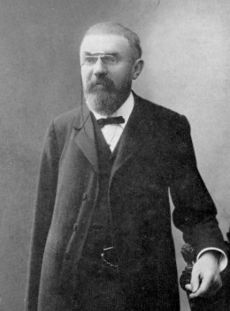
\includegraphics[height=\the\HauteurDesPhotos]{Poincare2}&
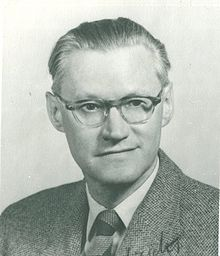
\includegraphics[height=\the\HauteurDesPhotos]{Friedrichs}&
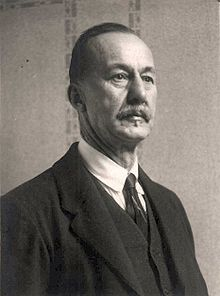
\includegraphics[height=\the\HauteurDesPhotos]{Wirtinger}&
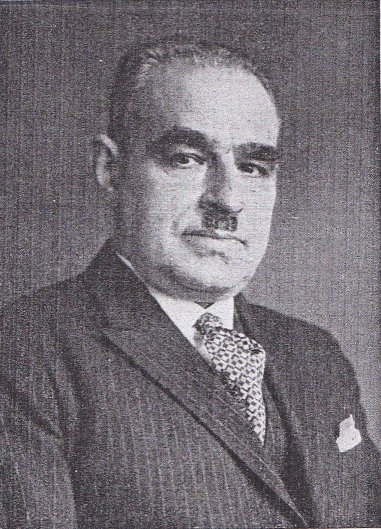
\includegraphics[height=\the\HauteurDesPhotos]{Korn}\\
Poincaré&Friedrichs&Wirtinger&Korn%
\end{tabular}}
\vskip7pt
\ImageADroite{%
Il est plus connu comme pionnier
des télécommunications, plus précisément comme l'inventeur de la téléphotographie. Il met au
point un téléautographe, un système de transmission des images fixes à distance, par le biais
du fil télégraphique, en recourant aux propriétés photoélectriques du sélénium.
}
\end{histoire}
